\documentclass[11pt]{article}
\usepackage[margin=1in, top=1in]{geometry}
\usepackage[all]{nowidow}
\usepackage[hyperfigures=true, hidelinks, pdfhighlight=/N]{hyperref}
\usepackage[separate-uncertainty=true, group-digits=false]{siunitx}
\usepackage{graphicx,amsmath,physics,tabto,float,amssymb,pgfplots,verbatim,tcolorbox}
\usepackage{listings,xcolor,subfig,caption,import,wrapfig,enumitem}
\usepackage[version=4]{mhchem}
\usepackage[noabbrev]{cleveref}
\newcommand{\creflastconjunction}{, and\nobreakspace}
\definecolor{stringcolor}{HTML}{C792EA}
\definecolor{codeblue}{HTML}{2162DB}
\definecolor{commentcolor}{HTML}{4A6E46}
\captionsetup{font=small, belowskip=0pt}
\lstdefinestyle{appendix}{
    basicstyle=\ttfamily\footnotesize,commentstyle=\color{commentcolor},keywordstyle=\color{codeblue},
    stringstyle=\color{stringcolor},showstringspaces=false,numbers=left,upquote=true,captionpos=t,
    abovecaptionskip=12pt,belowcaptionskip=12pt,language=Python,breaklines=true,frame=single}
\lstdefinestyle{inline}{
    basicstyle=\ttfamily\footnotesize,commentstyle=\color{commentcolor},keywordstyle=\color{codeblue},
    stringstyle=\color{stringcolor},showstringspaces=false,numbers=left,upquote=true,frame=tb,
    captionpos=b,language=Python}
\renewcommand{\lstlistingname}{Appendix}
\pgfplotsset{compat=1.17}

\begin{document}

\begin{center}
    \textbf{CP Tut 1}\hspace{2in}\textbf{KDSMIL001}\hspace{2in}\textbf{23-04-2022}
\end{center}

\begin{enumerate}
    \item \begin{enumerate}
        \item Using the method outlined on page 33 of the notes, we were able to simulate the decay of $N$ nuclei with an activity of $\Lambda=\SI{1.2}{\per\second}$. Running that simulation a number of times and noting how many decays occurred in each counting interval, for both 10s and 1s counting intervals, we were able to produce the plots in \cref{fig:q1ai,fig:q1aii}. Both times the simulation was run 1000 times.
        
        The means were found to be 1.205 with standard deviation 1.109 for \SI{1}{\second} and 11.243 with standard deviation 3.038 for \SI{10}{\second}. The expected mean is $\Lambda T$ where $T$ is the counting interval so with their respective standard deviations, they are reasonably close to the expected value.
        
        \begin{figure}[h]
            \begin{center}
                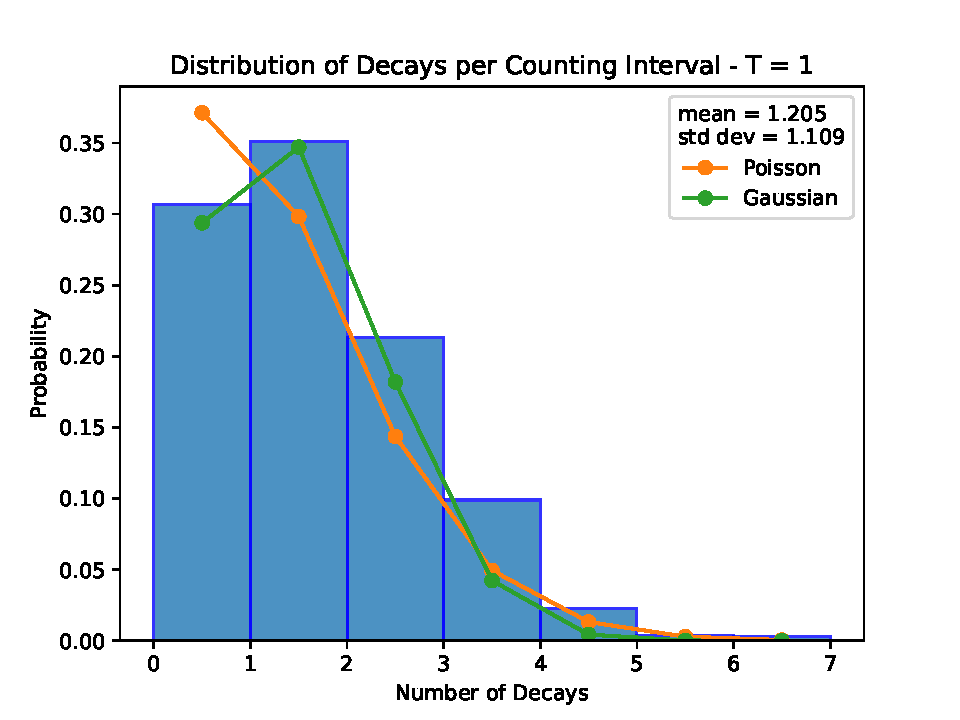
\includegraphics[width=0.6\textwidth]{Plots/q1ai.pdf}
                \caption{Distribution of decays per counting interval for $T=\SI{1}{\second}$, normalised and plotted with the Poisson and Gaussian distributions of the same mean and standard deviation. Simulation run 1000 times.}
                \label{fig:q1ai}
            \end{center}
        \end{figure}
        
        \begin{figure}[h]
            \begin{center}
                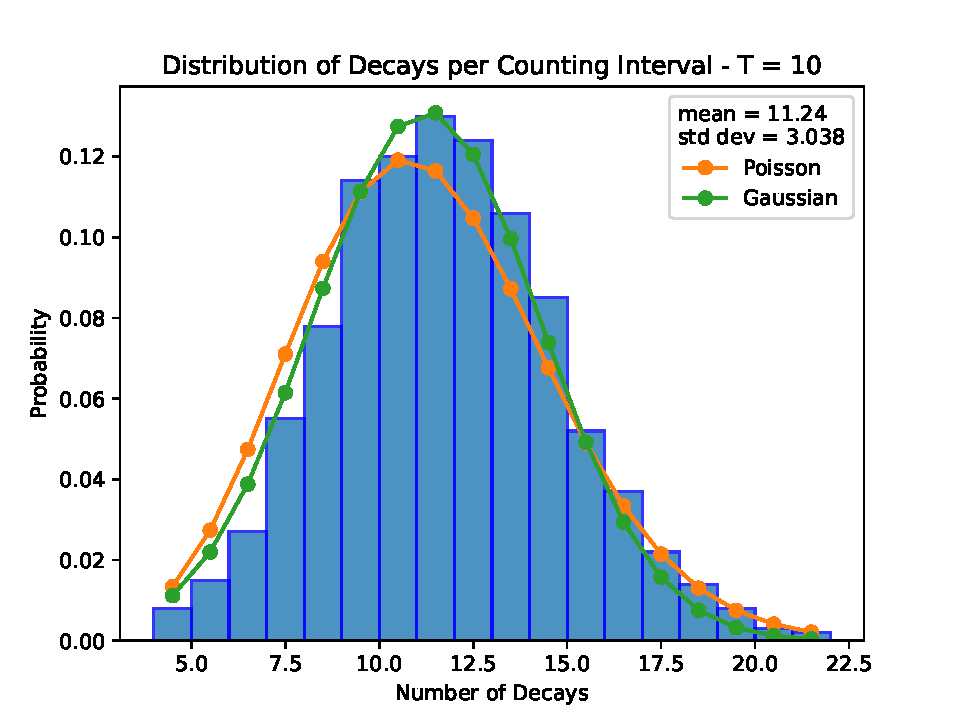
\includegraphics[width=0.6\textwidth]{Plots/q1aii.pdf}
                \caption{Distribution of decays per counting interval for $T=\SI{10}{\second}$, normalised and plotted with the Poisson and Gaussian distributions of the same mean and standard deviation. Simulation run 1000 times.}
                \label{fig:q1aii}
            \end{center}
        \end{figure}

        \item Along with the results of 1. a), \cref{fig:q1ai,fig:q1aii} show the comparison between the histograms and both a Poisson distribution as well as a Gaussian distribution. The mean used to plot both, as well as the standard deviation for the Gaussian, was drawn from the data itself. 
        
        We can see in both cases that the data is best modelled by the Gaussian distribution, which is not what we expect. For such low means, we expect the Poisson distribution to not be modelled well by the Gaussian, and we expect the data to follow a Poissonian distribution. The standard deviation of the data seems to suggest a Poissonian distribution, as both are close the the square root of the mean, but the plots suggest otherwise.

        \item In order to investigate the distribution of times between successive decays of the nuclei, we chose a counting interval of \SI{10}{\second} and ran the simulation 1000 times. Each time a decay occurred, the current time in the simulation was noted and if no decays had happened in the time step, the time since the last decay was calculated and added to an array. If there had already been a decay in that time step, the decay was ignored in order to avoid an interval of 0 seconds. The distribution resulting from this analysis, along with the expected form of an exponential distribution, is shown in \cref{fig:q1c}. 
        
        In order to work out the expected mean, we can think about $\Lambda$ telling us that we expect, on average, 1.2 decays every second, so the time between decays should be $1/\Lambda$, or \SI{0.833}{\second}. Looking at the mean in \cref{fig:q1c}, we find it to be \SI{0.801}{\second}. Throughout all our testing it was consistently lower than expected. We are not sure why this is.

        \begin{figure}[h]
            \begin{center}
                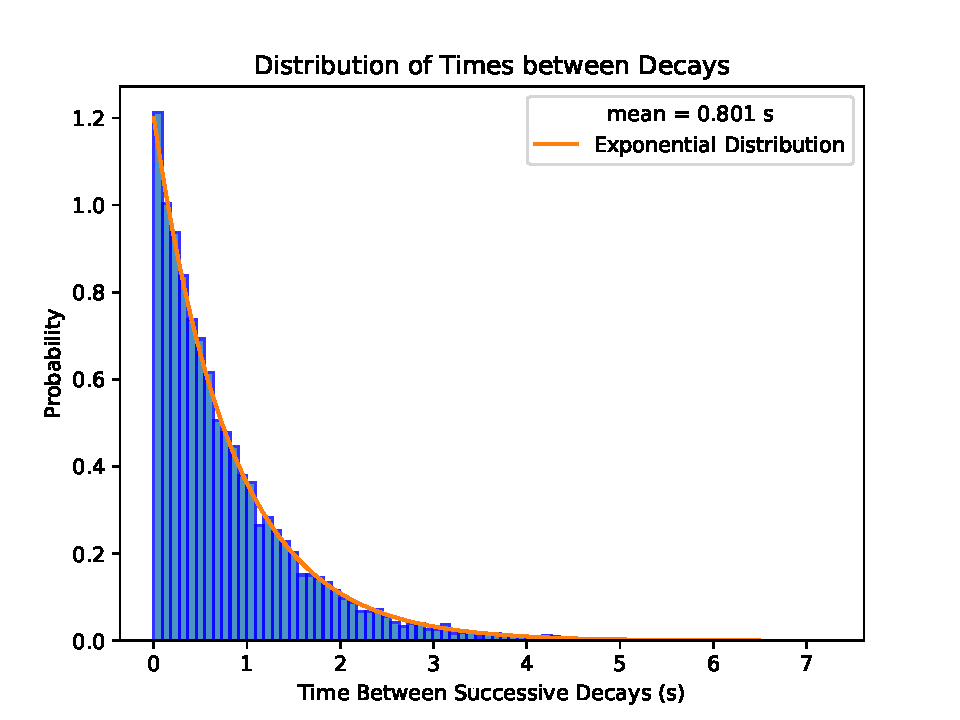
\includegraphics[width=0.6\textwidth]{Plots/q1c.pdf}
                \caption{Distribution of times between successive decays, ignoring decays that happen in the same time step. Plotted with the histogram is the exponential distribution with $\lambda=\Lambda$, the activity.}
                \label{fig:q1c}
            \end{center}
        \end{figure}
    \end{enumerate}

    \item \begin{enumerate}
        \item In order to use the transformation method, we integrated each probability distribution and rearranged to find $y_i$ in terms of the uniformly distributed $x_i$:
        \begin{enumerate}[label=\roman*)]
            \item \label{itm:q2ai}
            \begin{align*}
                x_i &=\int_{-\frac{\pi}{4}}^{y_i}\cos(2y')dy'\\
                &=\frac 12 (\sin(2y_i)+1)\\
                \implies y_i&=\frac{1}{2}\arcsin(2x_i-1)
            \end{align*}

            \item \label{itm:q2aii}
            \begin{align*}
                x_i&=\int_2^{y_i}\frac{1}{\sqrt 8 - \sqrt 3}\frac{y'}{\sqrt{y'^2-1}}dy'\\
                &=\frac{1}{\sqrt 8 - \sqrt 3}\left(\sqrt{y_i^2-1}-\sqrt 3\right)\\
                \implies y_i&=\sqrt{(x_i(\sqrt{8}-\sqrt{3})+\sqrt{3})^2+1}
            \end{align*}

            \item \label{itm:q2aiii}
            \begin{align*}
                x_i&=\int_1^{y_i}\frac{1}{\sqrt 8}\frac{y'}{\sqrt{y'^2-1}}dy'\\
                &=\sqrt{\frac{y_i^2-1}{8}}\\
                \implies y_i&=\sqrt{8x_i^2+1}
            \end{align*}
        \end{enumerate}
        Then by simply generating 500 000 random numbers in $[0,1)$ and feeding them through the equations found above, we could generate 500 000 numbers distributed according to the respective probability distribution.

        \begin{figure}[H]%
            \centering
            \subfloat[\centering Uniform distribution of $x_i$ values]{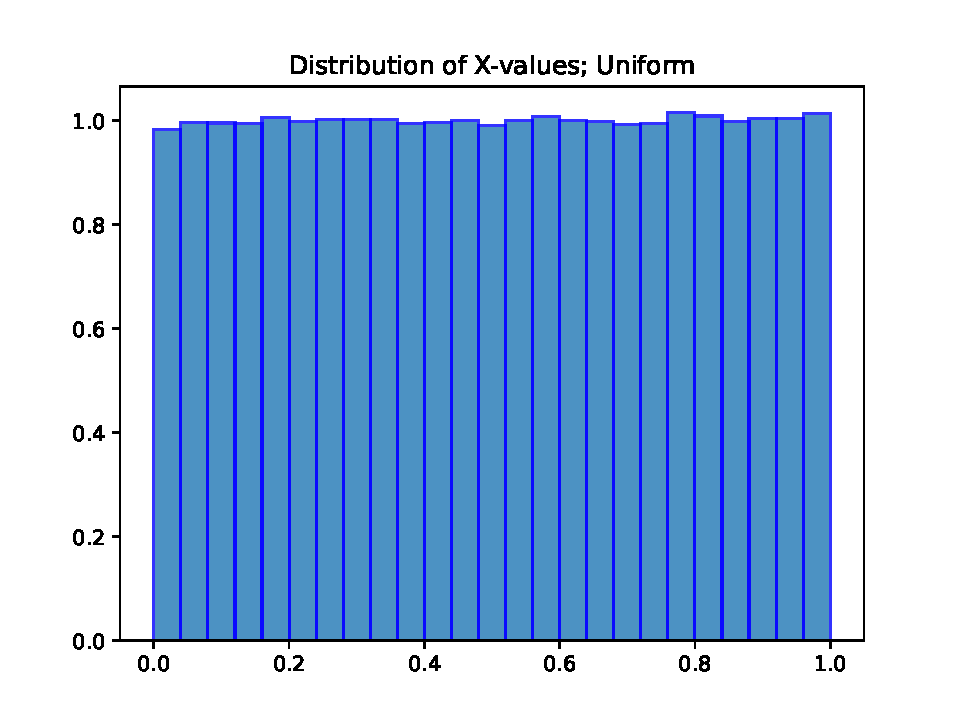
\includegraphics[width=.45\textwidth]{Plots/q2aix.pdf}}
            \,
            \subfloat[\centering Distribution of $y_i$ values]{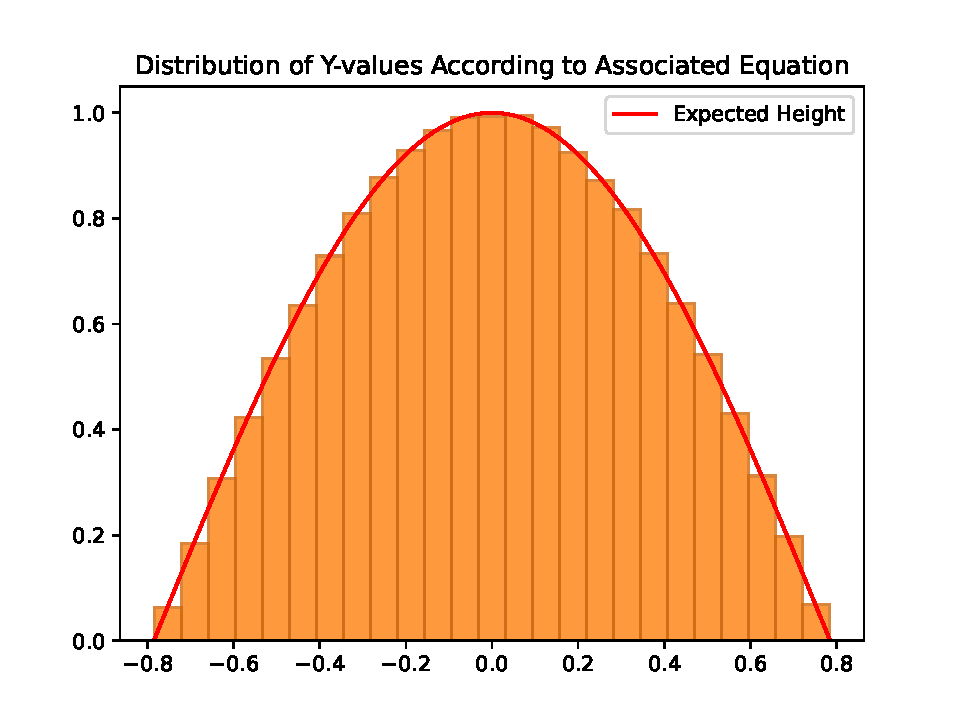
\includegraphics[width=.45\textwidth]{Plots/q2aiy.pdf}}
            \caption{The uniform distribution of numbers in $[0,1)$ alongside the $y_i$ values generated from them using the transformation method, according to $p(y)=\cos(2y)$. Plotted with the transformed distribution is the expected probability distribution. Each distribution is split into 25 bins. 500 000 numbers were generated.}
            \label{fig:q2ai}
        \end{figure}

        \begin{figure}[H]%
            \centering
            \subfloat[\centering Uniform distribution of $x_i$ values]{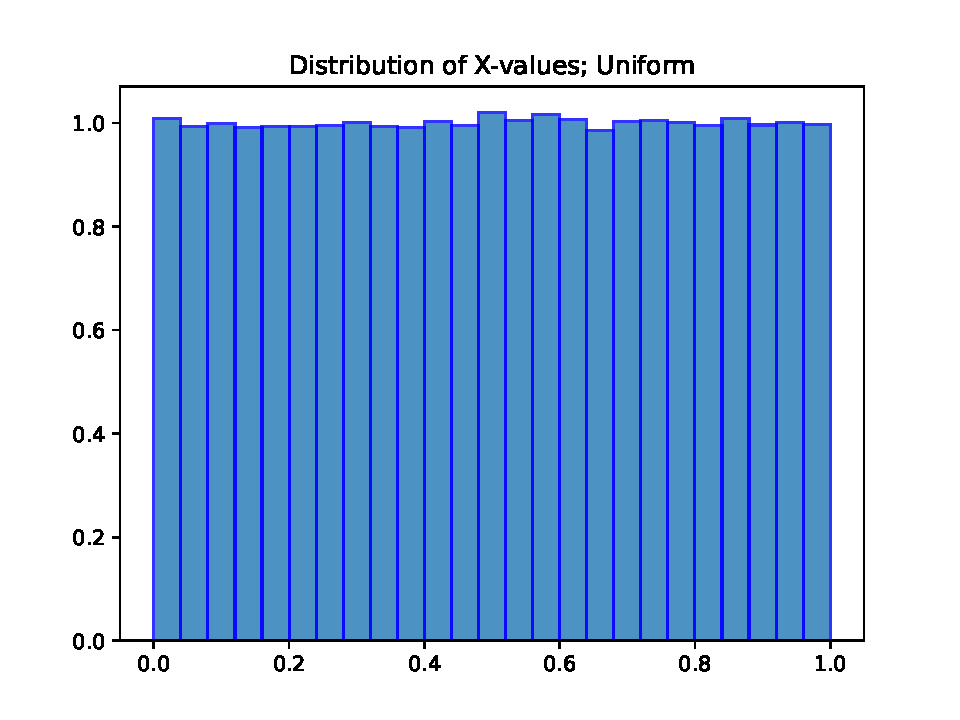
\includegraphics[width=.45\textwidth]{Plots/q2aiix.pdf}}
            \,
            \subfloat[\centering Distribution of $y_i$ values]{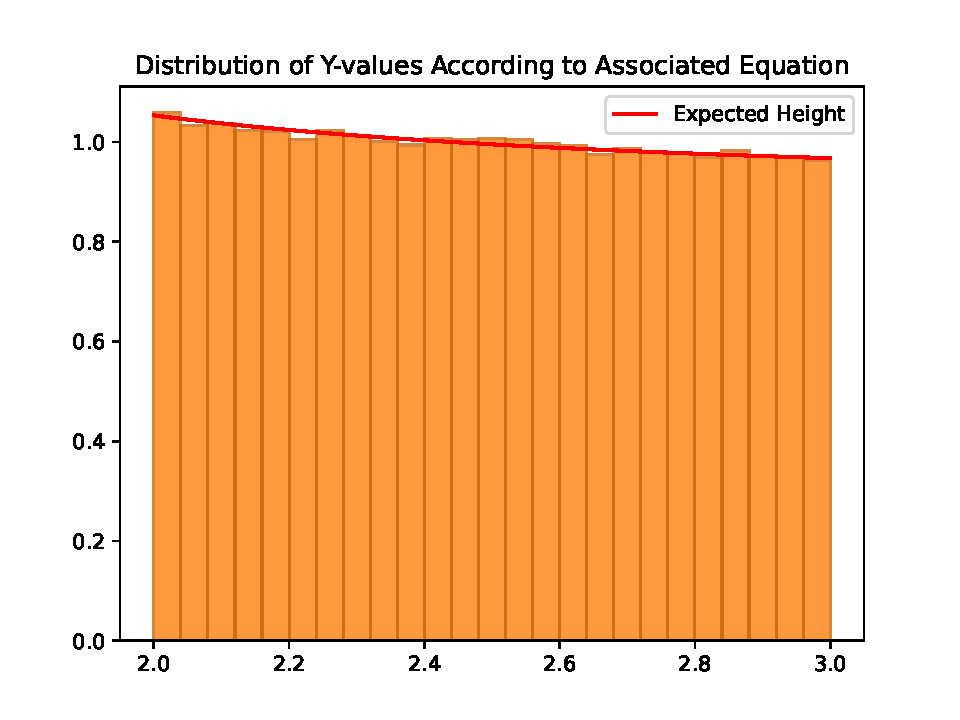
\includegraphics[width=.45\textwidth]{Plots/q2aiiy.pdf}}
            \caption{The uniform distribution of numbers in $[0,1)$ alongside the $y_i$ values generated from them using the transformation method, according to $p(y)=\frac{1}{\sqrt 8 - \sqrt 3}\frac{y}{\sqrt{y^2-1}}$. Plotted with the transformed distribution is the expected probability distribution. Each distribution is split into 25 bins. 500 000 numbers were generated.}
            \label{fig:q2aii}
        \end{figure}

        \begin{figure}[H]%
            \centering
            \subfloat[\centering Uniform distribution of $x_i$ values]{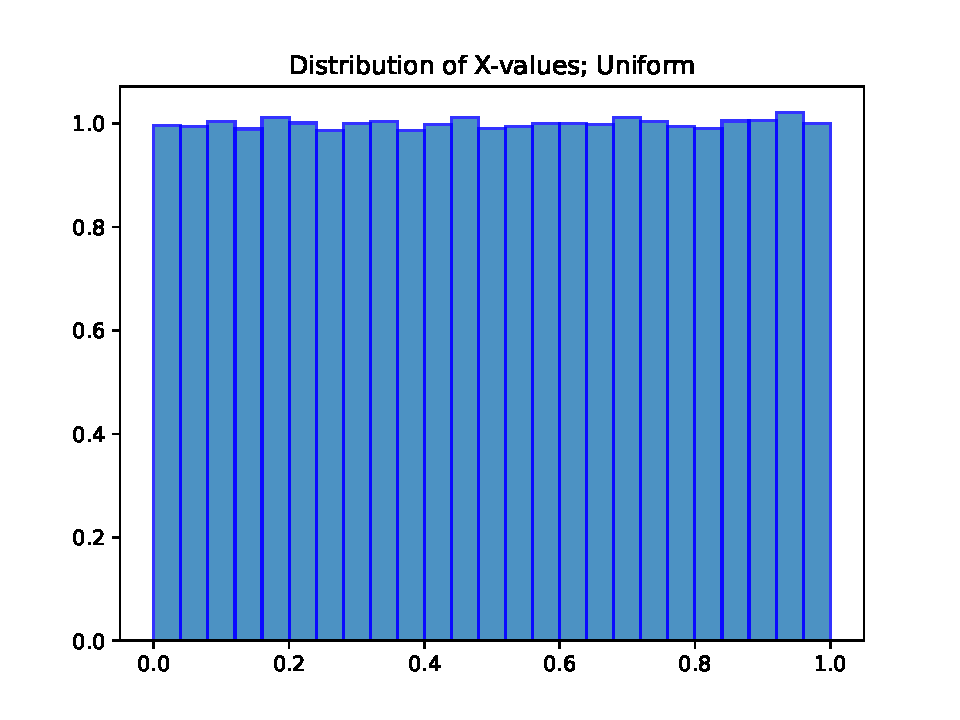
\includegraphics[width=.45\textwidth]{Plots/q2aiiix.pdf}}
            \,
            \subfloat[\centering Distribution of $y_i$ values]{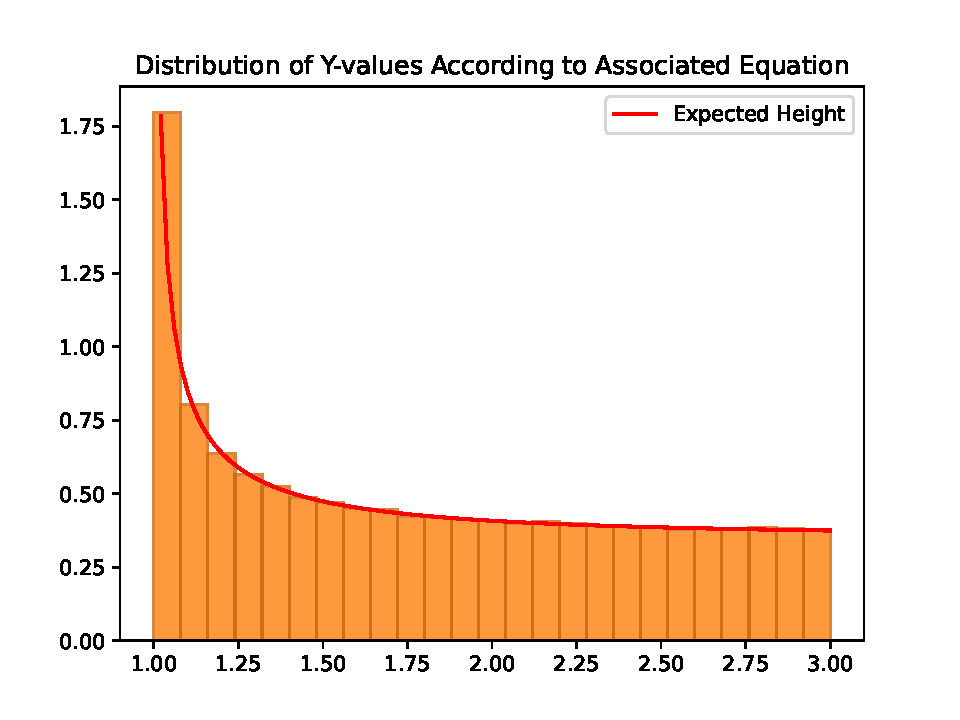
\includegraphics[width=.45\textwidth]{Plots/q2aiiiy.pdf}}
            \caption{The uniform distribution of numbers in $[0,1)$ alongside the $y_i$ values generated from them using the transformation method, according to $p(y)=\frac{1}{\sqrt 8}\frac{y}{\sqrt{y^2-1}}$. Plotted with the transformed distribution is the expected probability distribution. Each distribution is split into 25 bins. 500 000 numbers were generated.}
            \label{fig:q2aiii}
        \end{figure}

        We can see in each case that the transformation method worked well, accurately approximating the respective probability distribution. 

        \item Next, we aimed to use the rejection method to generate 500 000 random numbers according to the distribution in \cref{fig:q2ai}: $p(y)=\cos(2y)$. To do this we first find the maximum value of $p(y)$ in the interval of interest, then generate a pair of numbers corresponding to a coordinate in the box bounded by the interval and the maximum value. If this coordinate falls within the distribution, it is accepted, otherwise it is rejected and we try again. This is repeated until the required amount of numbers $y_i$ are generated, in our case 500 000. 
        
        In order to speed up computation, we wanted to avoid generating a random number at each iteration, so a set of random numbers is generated at the start and then looped over to find those that will be accepted. This requires knowing how many, on average, will be accepted by the algorithm. This can be calculated using
        \begin{equation}
            P(\text{accept}) = \frac{\int_a^b p(y) dy}{p_{\text{max}}(b-a)}=\frac{1}{p_{\text{max}}(b-a)}
        \end{equation}
        The last step assumes the probability distribution is normalised. With this, we can generate $NP(\text{accept})$ random numbers, multiplied by 1.5 to be safe, and be certain that we will accept at least $N$ in the process.

        Using this method, we produced the plot in \cref{fig:q2b}, finding that the method approximated the true distribution fairly well. 

        \begin{figure}[h]
            \begin{center}
                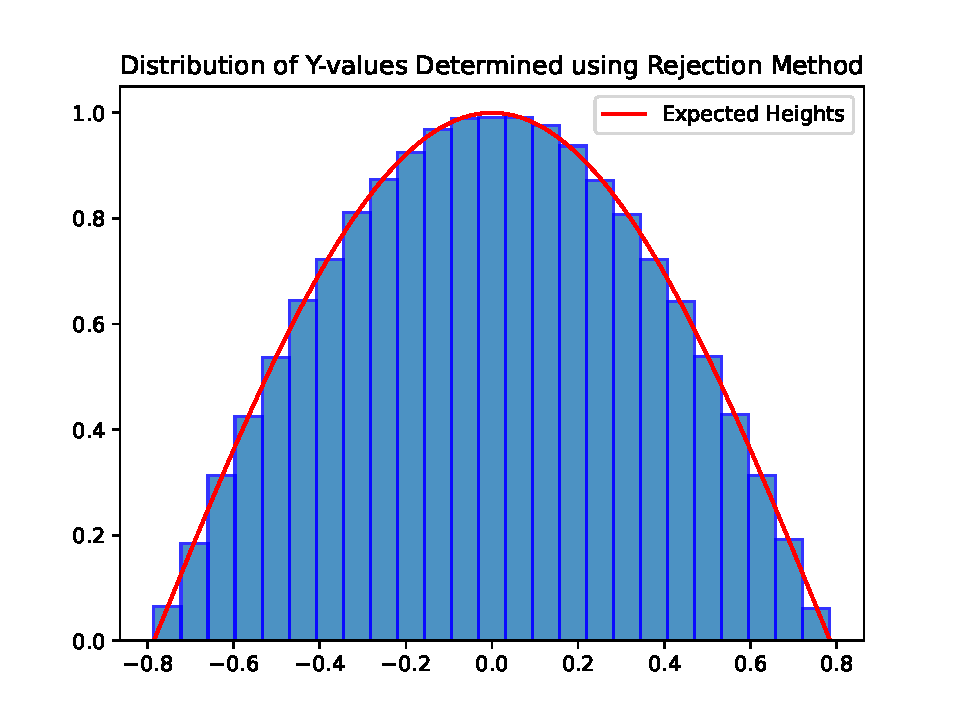
\includegraphics[width=.6\textwidth]{Plots/q2b.pdf}
                \caption{Random numbers distributed according to $p(y)=\cos(2y)$ using the rejection method. 500 000 numbers were generated. The data is histogrammed into 25 bins. The expected form of the distribution is plotted along with the histogram.}
                \label{fig:q2b}
            \end{center}
        \end{figure}
        
        \item The rejection method could be used to generate the distribution in \cref{itm:q2aii} as it is fairly flat and as such would have a relatively high acceptance rate. On the other hand, \cref{itm:q2aiii} would not be able to be generated using rejection, at least not easily. It blows up at $y=1$ and as such would have a maximum in the interval of $\infty$. This would effectively make the acceptance rate 0. Even ignoring that end of the interval wouldn't help as near to it the value of the distribution would still be very large, leading to a low acceptance rate.
    \end{enumerate}

    \item 
\end{enumerate}

% q3 results
% pHit: 0.027792733488535566
% rejectionRate 0.788316
% rejection average: 12.458407178501192
% combo average: 12.48345169474772
% number of combo above 100: 205949
% Time taken for Rejection Method: 4.492590665817261
% Time taken for Combination Method: 0.4290454387664795

\end{document}